% Created 2024-01-31 qua 13:47
% Intended LaTeX compiler: xelatex
\documentclass[11pt]{article}
\usepackage{graphicx}
\usepackage{longtable}
\usepackage{wrapfig}
\usepackage{rotating}
\usepackage[normalem]{ulem}
\usepackage{amsmath}
\usepackage{amssymb}
\usepackage{capt-of}
\usepackage{hyperref}
\usepackage{minted}
\usepackage{bbm}
\usepackage{amsfonts,amsmath,mathtools}
\usepackage[linesnumbered,ruled]{algorithm2e}
\usepackage{dsfont}
\usepackage{graphicx}
\usepackage{caption}
\usepackage{subcaption}
\usepackage{multirow}
\usepackage{natbib}
\newcommand{\res}{\mathbf{r}}
\newcommand{\w}{\mathbf{w}}
\newcommand{\m}{\mathbf{m}}
\newcommand{\x}{\mathbf{x}}
\newcommand{\C}{\mathbb{C}}
\newcommand{\E}{\mathbb{E}}
\newcommand{\N}{\mathrm{N}}
\newtheorem{assumption}{Assumption}[section]
\newtheorem{theorem}{Theorem}[section]
\newcommand{\indep}{\perp \!\!\! \perp}
\author{Rafael Alcantara\thanks{rafaelca10@al.insper.edu.br}}
\date{\today}
\title{Previous RDD Papers}
\hypersetup{
 pdfauthor={Rafael Alcantara},
 pdftitle={Previous RDD Papers},
 pdfkeywords={},
 pdfsubject={},
 pdfcreator={Emacs 29.1 (Org mode 9.6.6)}, 
 pdflang={English}}
\begin{document}

\maketitle
\tableofcontents

\section{Previous RDD papers}
\label{sec:orgbef6825}
It is worth noting that most of the papers write the DGPs in
terms of \(E[Y_1|X]=\mu_1(x)\) and \(E[Y_0|X]=\mu_0(x)\). While
this makes sense from the perspective that most methods
consist of approximating each function and taking their
differences at \(x=c\), I rewrite the DGPs in terms of a
prognostic and treatment function, \(\mu(x)\) and \(\tau(x)\)
respectively, as this makes more sense from a BCF
perspective.
\subsection{Without W}
\label{sec:org925f748}
\subsubsection{IK2012}
\label{sec:org20d4a96}
\cite{imbens2012optimal} consider 4 different DGPs. For every
DGP, they consider \(n=500\) and sample \(X\) from \(X \sim 2
\mathcal{B}(2,4) - 1\), \(Z = \mathbf{1}(X \geq 0)\) and
\(\varepsilon \sim \mathcal{N}(0,0.1295^2)\). For each DGP,
the prognostic and treatment effect functions are defined
as:

\begin{enumerate}
\item Based on \cite{lee2008randomized}\footnote{Every simulation based on ``Lee data'' refers to this}:
\begin{itemize}
\item \(\mu(x) = 0.48 + 1.27 x + 7.18 x^2 + 20.21 x^3 + 21.54
     x^4 + 7.33 x^5\)
\item \(\tau(x) = 0.04 - 0.43 x - 10.18 x^2 - 12.22 x^3 - 12.53
     x^4 - 3.77 x^5\)
\end{itemize}
\item Quadratic on X:
\begin{itemize}
\item \(\mu(x) = 3 x^2\)
\item \(\tau(x) = x ^2\)
\end{itemize}
\item Constant ATE:
\begin{itemize}
\item \(\mu(x) = 0.42 + 0.84 x - 3 x^2 + 7.99 x^3 - 9.01 x^4 +
     3.56 x^5\)
\item \(\tau(x) = 0.1\)
\end{itemize}
\item Constant ATE and curvature at the threshold is zero at
both sides:
\begin{itemize}
\item \(\mu(x) = 0.42 + 0.84 x + 7.99 x^3 - 9.01 x^4 + 3.56
     x^5\)
\item \(\tau(x) = 0.1\)
\end{itemize}
\end{enumerate}

This is what each DGP looks like:

\begin{center}
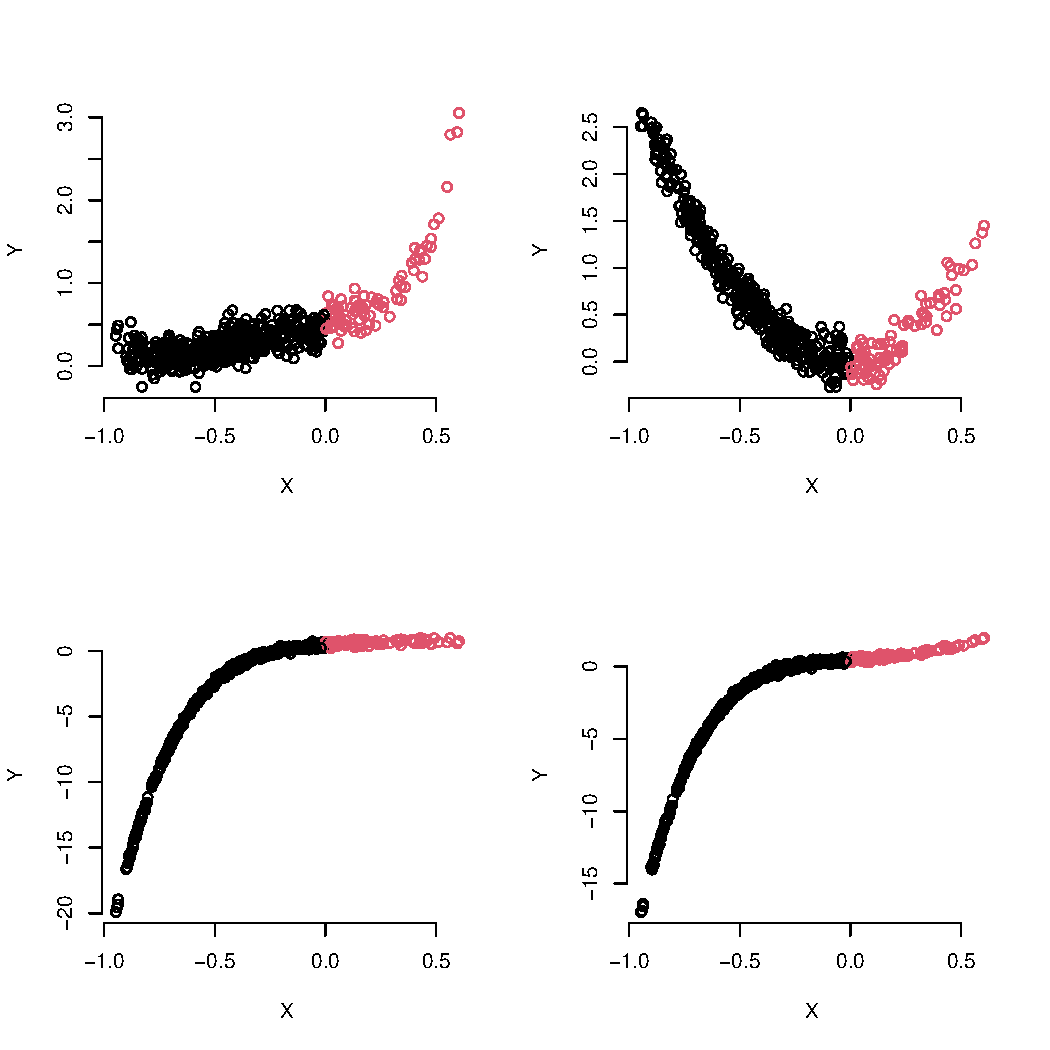
\includegraphics[width=.9\linewidth]{IK2012.pdf}
\end{center}

\subsubsection{CCT2014}
\label{sec:org9a19808}
\cite{calonico2014robust} repeat \(n\), \(X\) and \(\varepsilon\)
from \cite{imbens2012optimal}. Their regression functions
follow\footnote{Simulations detailed in supplemental material}:

\begin{enumerate}
\item Lee data
\item Based on \cite{ludwig2007does}\footnote{Every simulation based on ``LM data'' refers to this}:
\begin{itemize}
\item \(\mu(x) = 3.71 + 2.30 x + 3.28 x^2 + 1.45 x^3 + 0.23
     x^4 + 0.03 x^5\)
\item \(\tau(x) = -3.45 + 16.19 x - 58.09 x^2 + 72.85 x^3 -
     45.25 x^4 + 9.8 x^5\)
\end{itemize}
\item Variation of Lee data
\begin{itemize}
\item \(\mu(x) = 0.48 + 1.27 x - 3.59 x^2 + 14.147 x^3 +
     23.694 x^4 + 10.995 x^5\)
\item \(\tau(x) = 0.04 - 0.43 x + 3.29 x^2 - 16.544 x^3 -
     24.595 x^4 - 7.435 x^5\)
\end{itemize}
\end{enumerate}

This is what each DGP looks like:

\begin{center}
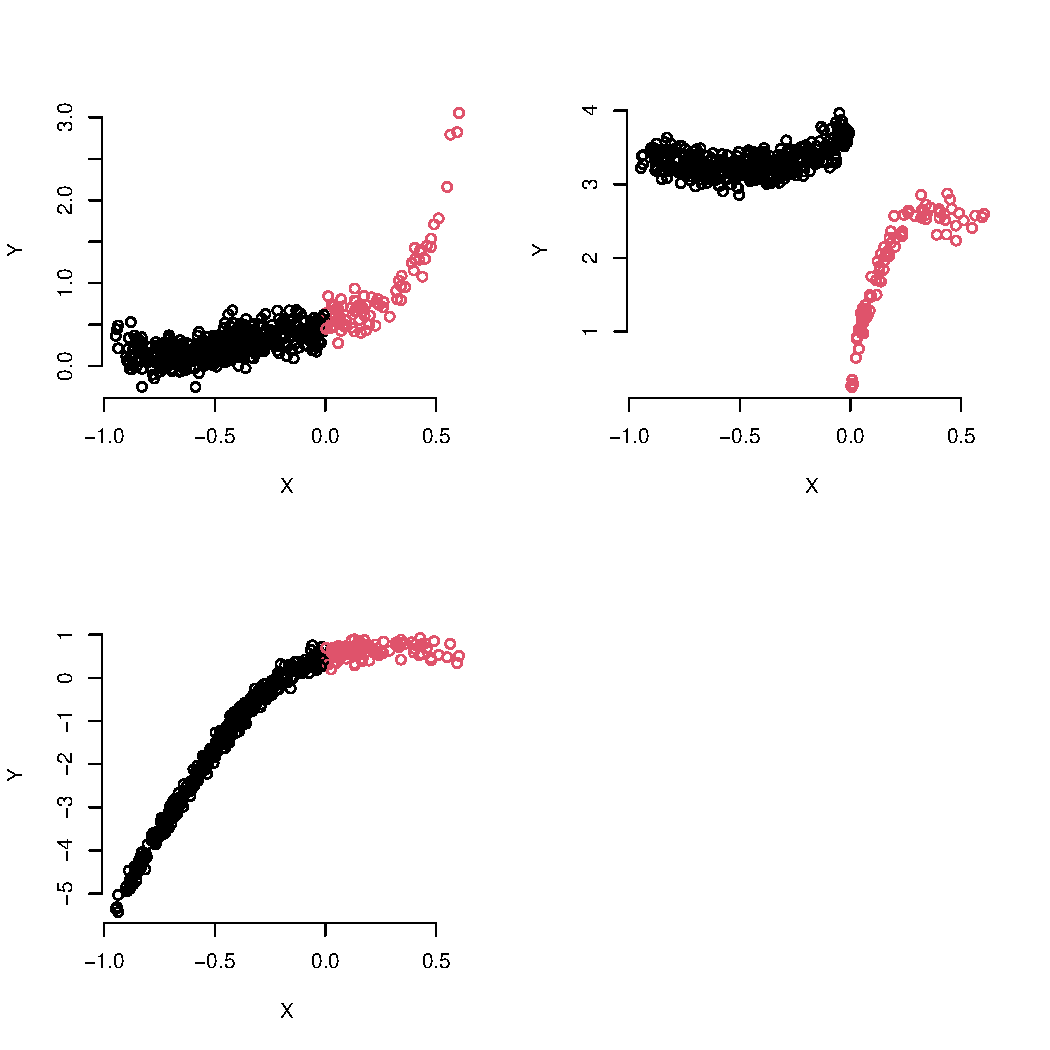
\includegraphics[width=.9\linewidth]{CCT2014.pdf}
\end{center}

\subsubsection{BRBM2019}
\label{sec:orgce3953f}
\cite{branson2019nonparametric} fit two different GP
regressions to treated and untreated units. They generate
1000 samples of 7 different DGPs. In each case, \(n\), \(X\) and
\(\varepsilon\) are the same as \cite{imbens2012optimal}. The
regression functions are the same as \cite{imbens2012optimal}
and \cite{calonico2014robust} plus one additional setup:

\begin{enumerate}
\item Cubic functions:
\begin{itemize}
\item \(\mu(x) = 3 x^3\)
\item \(\tau(x) = x^3\)
\end{itemize}
\end{enumerate}

The DGPs look like this:

\begin{center}
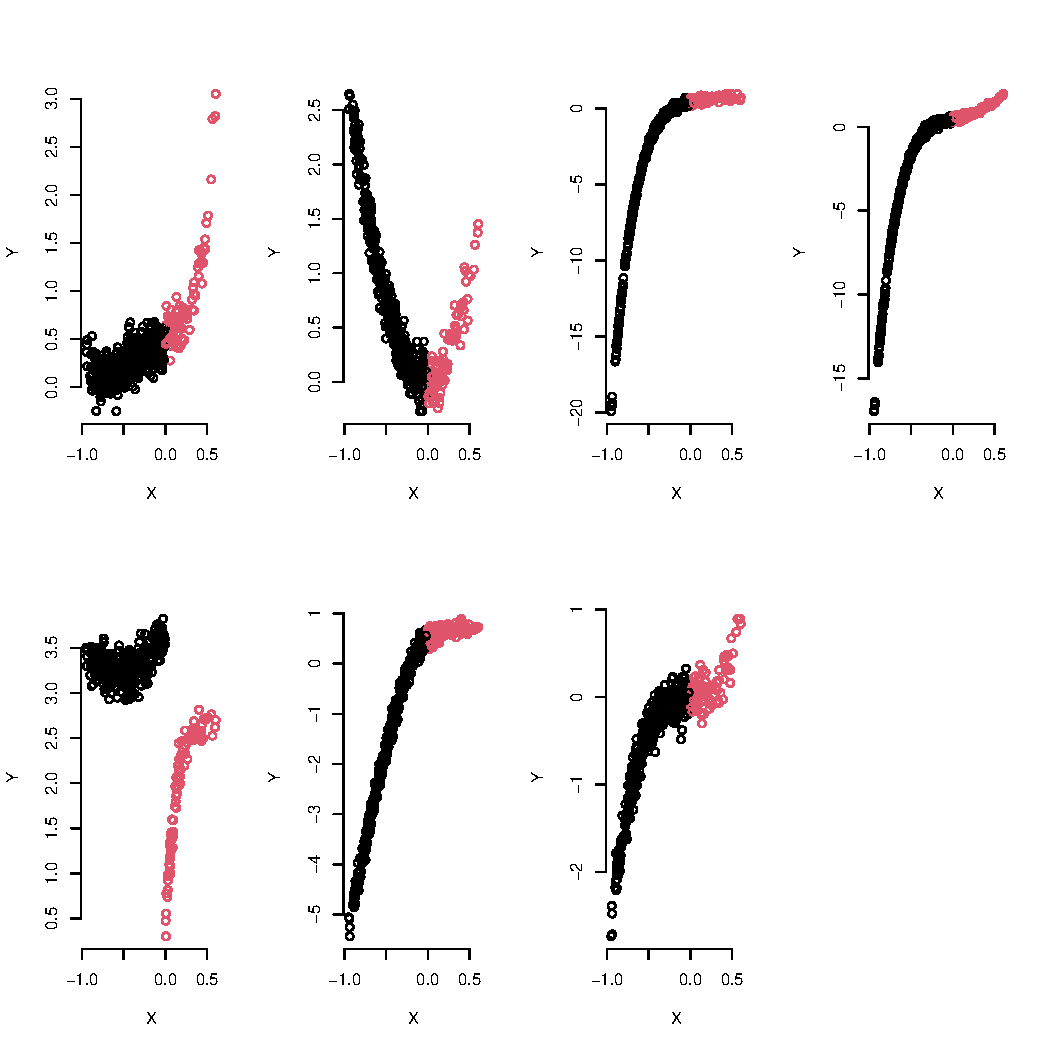
\includegraphics[width=.9\linewidth]{BRBM2019.pdf}
\end{center}

\subsubsection{CCF2020}
\label{sec:org73056eb}
\cite{calonico2020optimal} consider a variation of the LM data
with a different cutoff and higher error variance, but same
parameters for \(\mu\) and \(\tau\).
\subsection{With W}
\label{sec:org349a438}
\subsubsection{CGS2023}
\label{sec:org6729e1e}
\cite{chib2023nonparametric} analyzes two DGPs. First, the
classic Lee data with t-distributed erros instead of
Gaussian errors. They also consider a setup with
nonparametric errors as follows. \(\mu,\tau\) are an extension
of the Lee data DGP that also includes \(W\) but in such a way
that there still are no heterogeneous effects. For this DGP
they also propose a more intricate error structure. The DGP
is:

\begin{equation}
  \begin{split}
    \mu(x,w) &= 0.48 + 1.27 x + 7.18 x^2 + 20.21 x^3 + 21.54 x^4 + 7.33 x^5 + h(w) + \varepsilon_{\mu}\\
    \tau(x,w) &= 0.04 - 0.43 x - 10.18 x^2 - 12.22 x^3 - 12.53 x^4 - 3.77 x^5 + \varepsilon_{\tau}\\
    h(w) &= \frac{\sin(\pi w/2)}{1 + w^2(\text{sign}(w)+1)}\\
    w &\sim U(-\pi,\pi)\\
    \varepsilon_{\mu} &= \varepsilon_0\\
    \varepsilon_{\tau} &= \varepsilon_1 - \varepsilon_0.
  \end{split}
\end{equation}

The errors follow:

\begin{equation}
  \begin{split}
    F(\varepsilon_0) &= \sigma_0 F(\varepsilon)\\
    F(\varepsilon_1) &= \sigma_1 F(\varepsilon)\\
    F(\varepsilon) &= \frac{1}{3} \times \Phi(\varepsilon + 2.5) + \frac{1}{3} \times \Phi(\varepsilon) + \frac{1}{3} \times \Phi(\varepsilon - 2.5)\\
    \sigma_0 &= 0.1295\\
    \sigma_1 &= 0.2.
  \end{split}
\end{equation}

This is what that second DGP looks like:

\begin{center}
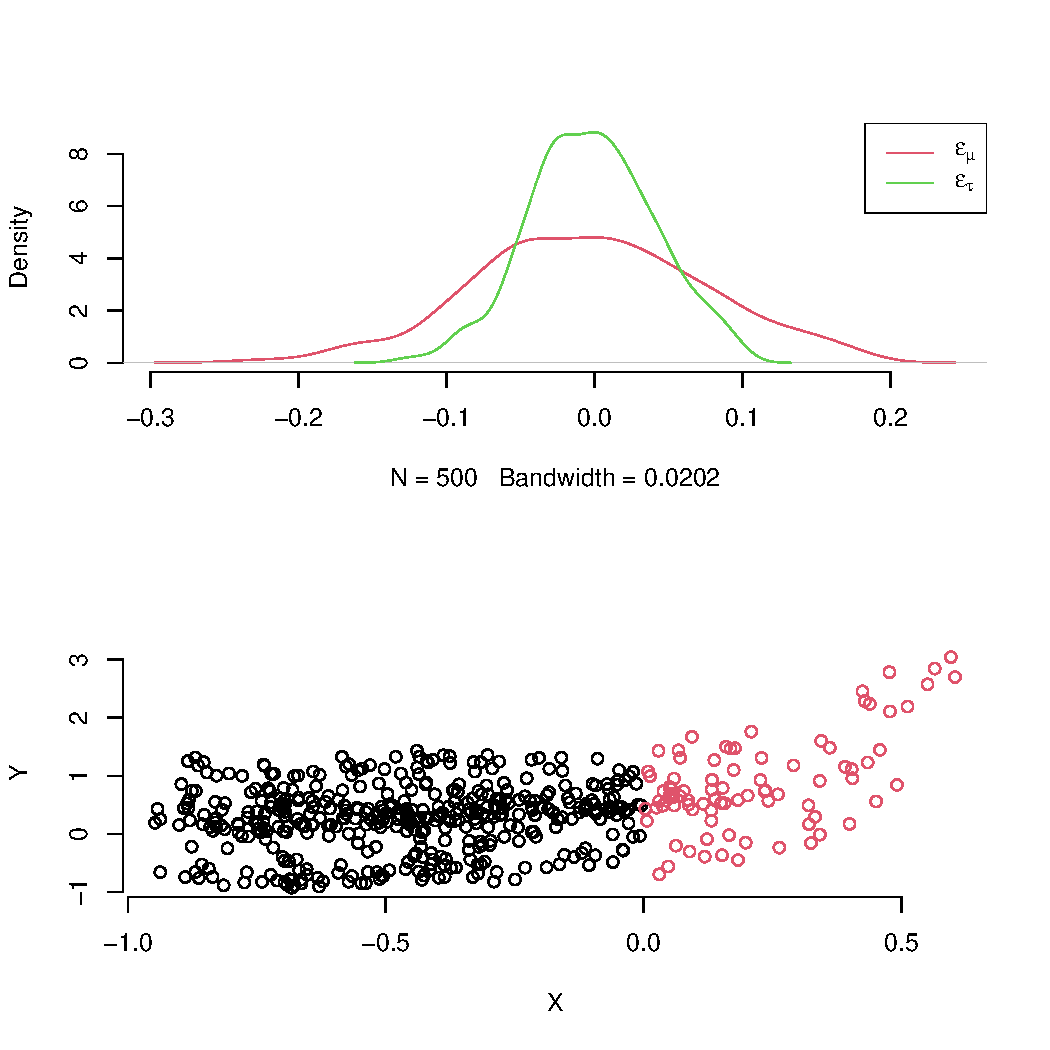
\includegraphics[width=.9\linewidth]{cgs2023.pdf}
\end{center}

\subsubsection{CCT2019}
\label{sec:org4281de9}
\cite{calonico2019regression}\footnote{\url{https://github.com/rdpackages-replication/CCFT\_2019\_RESTAT/blob/master/CCFT\_2019\_RESTAT\_simuls.do}} consider 4 variations of
the Lee data by adding a pre-determined binary covariate
(previous democratic share). Each model includes this
covariate differently. For DGP 1, the covariate is
irrelevant and the DGP is the same as the classic Lee data
DGP. For the others, the covariate is relevant. For all
three, \(X\) and \(W\) follow:

\begin{equation}
  \begin{split}
    w_r &= 0.49 + (1.06-0.45) x + (5.74-5.51) x^2 \\
    &+ (17.14-20.60) x^3 + (19.75-13.32) x^4 + (7.47-10.95) x^5 + \varepsilon_w\\
    w_l &= 0.49 + 1.06 x + 5.74 x^2 + 17.14 x^3 + 19.75 x^4 + 7.47 x^5 + \varepsilon_w\\
    y_r &= 0.38 + 0.63 x - 2.85 x^2 + 8.43 x^3 - 10.24 x^4 + 4.32 x^5 + 0.28 w_r + \varepsilon_y\\
    y_l &= 0.36 + 0.96 x + 5.47 x^2 + 15.28 x^3 + 15.87 x^4 + 5.14 x^5 + 0.22 w_l + \varepsilon_y\\
    \sigma_y &= 0.1295\\
    \sigma_w &= 0.13537.
  \end{split}
\end{equation}

This implies:

\begin{equation}
  \begin{split}
    y &= \mu(x,\varepsilon_w) + \tau(x,\varepsilon_w)z + \varepsilon_y\\
    \mu(x,\varepsilon_w) &= 0.47 + 1.19 x + 6.73 x^2 + 19.05 x^3 + 20.21 x^4 + 6.78 x^5 + 0.22 \varepsilon_w\\
    \tau(x,\varepsilon_w) &= 0.049 - 0.36 x - 0.87 x^2 - 10.35 x^3 - 27.85 x^4 - 2.78 x^5 + 0.06 \varepsilon_w.
  \end{split}
\end{equation}

What differs from one DGP to the other is the joint
distribution of \(\varepsilon_y,\varepsilon_w\):

\begin{enumerate}
\item DGP 2: \(\sigma_{yw} = 0.2692 \sigma_y \sigma_w\)
\item DGP 3: \(\sigma_{yw} = 0\)
\item DGP 4: \(\sigma_{yw} = 0.5384 \sigma_y \sigma_w\)
\end{enumerate}

In each case, \(\varepsilon_y,\varepsilon_w\) are sampled
jointly from a Gaussian with covariance:

\begin{equation}
  \Sigma = \begin{pmatrix}
    \sigma_y^2 & \sigma_{yw}\\
    \sigma_{yw} & \sigma_w^2
  \end{pmatrix}.
\end{equation}

This is what the data looks like:

\begin{center}
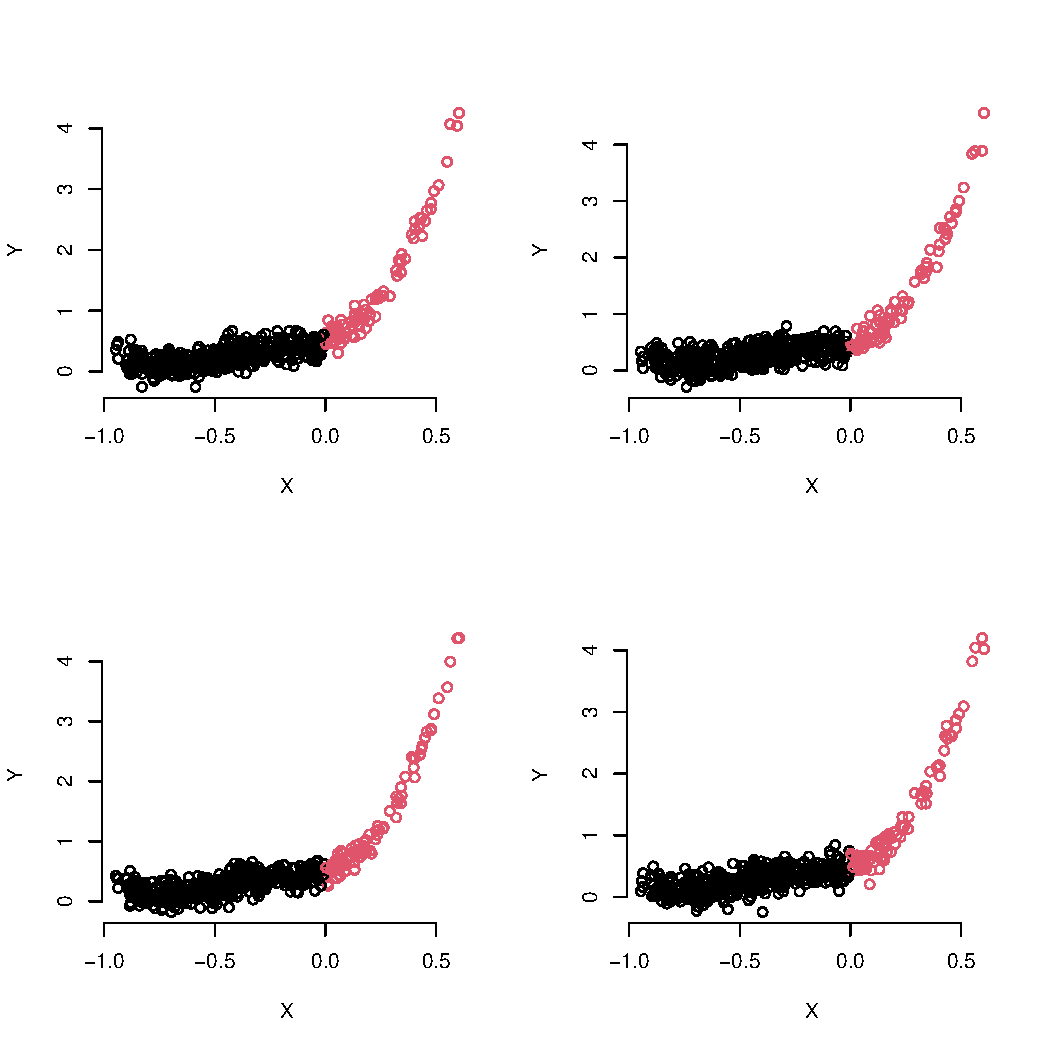
\includegraphics[width=.9\linewidth]{ccft2019.pdf}
\end{center}

\subsubsection{FH2019}
\label{sec:org7d400ea}
\cite{frolich2019including} analyze a setup where the
additional covariates might be discontinuous at the
cutoff. The DGP follows:

\begin{equation}
  \begin{split}
    X,U_1,U_2,U_3 &\sim \mathcal{N}(0,1)\\
    Z &= \mathbf{1}(X \geq 0)\\
    W_1 &= \alpha Z + 0.5 U_1\\
    W_2 &= \alpha Z + 0.5 U_2\\
    \mu(x,w) &= \beta(w_1+w_2) + \frac{\beta}{2}(w_1^2+w_2^2) + 0.5 x + 0.25 x^2\\
    \tau(x) &= 1 - 0.25 x\\
    y &= \mu(x,w) + \tau(x) z + u_3\\
    \alpha &\in \{0,0.2\}\\
    \beta &= 0.4.
  \end{split}
\end{equation}

This is what that DGP looks like for both values of
\(\alpha\):

\begin{center}
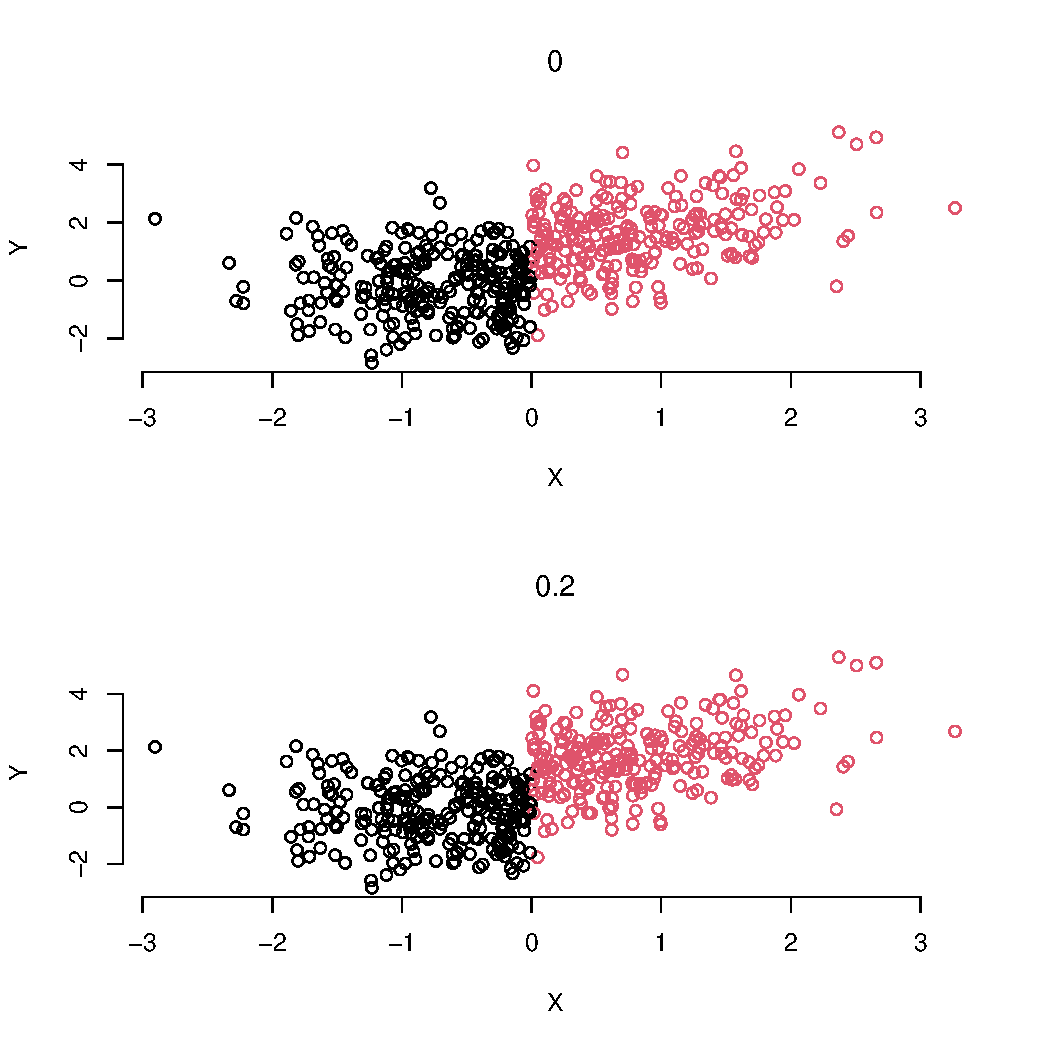
\includegraphics[width=.9\linewidth]{FH2019.pdf}
\end{center}

\subsubsection{KR2023}
\label{sec:org4489f39}
\cite{kreiss2021inference} also consider a polynomial DGP but
\(W,\varepsilon\) are sampled jointly.
\begin{equation}
  \begin{split}
    p &= 200\\
    X &\sim 2 \mathcal{B}(2,4) - 1\\
    Z &= \mathbf{1}(X \geq 0)\\
    (\varepsilon,W^T)^T &\sim \mathcal{N}(\mathbf{0},\Sigma)\\
    \Sigma &= \begin{pmatrix}
      \sigma^2_{\varepsilon} & \nu^T\\
      \nu & \sigma^2_W I_p
    \end{pmatrix}\\
    \mu(X,W) &= 0.36 + 0.96 X + 5.47 X^2 + 15.28 X^3 + 15.87 X^4 + 5.14 X^5 + 0.22 W^T \alpha\\
    \tau(X,W) &= 0.02 - 0.34 X - 8.31 X^2 - 6.86 X^3 - 26.11 X^4 - 0.83 X^5 + 0.06 W^T \alpha\\
    \sigma_{\varepsilon} &= 0.1295\\
    \sigma_W &= 0.1353\\
    \nu &\in \mathcal{R}^{200}, \quad \nu_k = \frac{0.8 \sqrt{6}\sigma^2_{\varepsilon}}{\pi k}\\
    \alpha &\in \mathcal{R}^{200}, \quad \alpha_k = \frac{2}{k^2}\\
    Y &= \mu(X,W) + \tau(X,W) Z + \varepsilon.
  \end{split}
\end{equation}

This is what the errors and data looks like:

\begin{center}
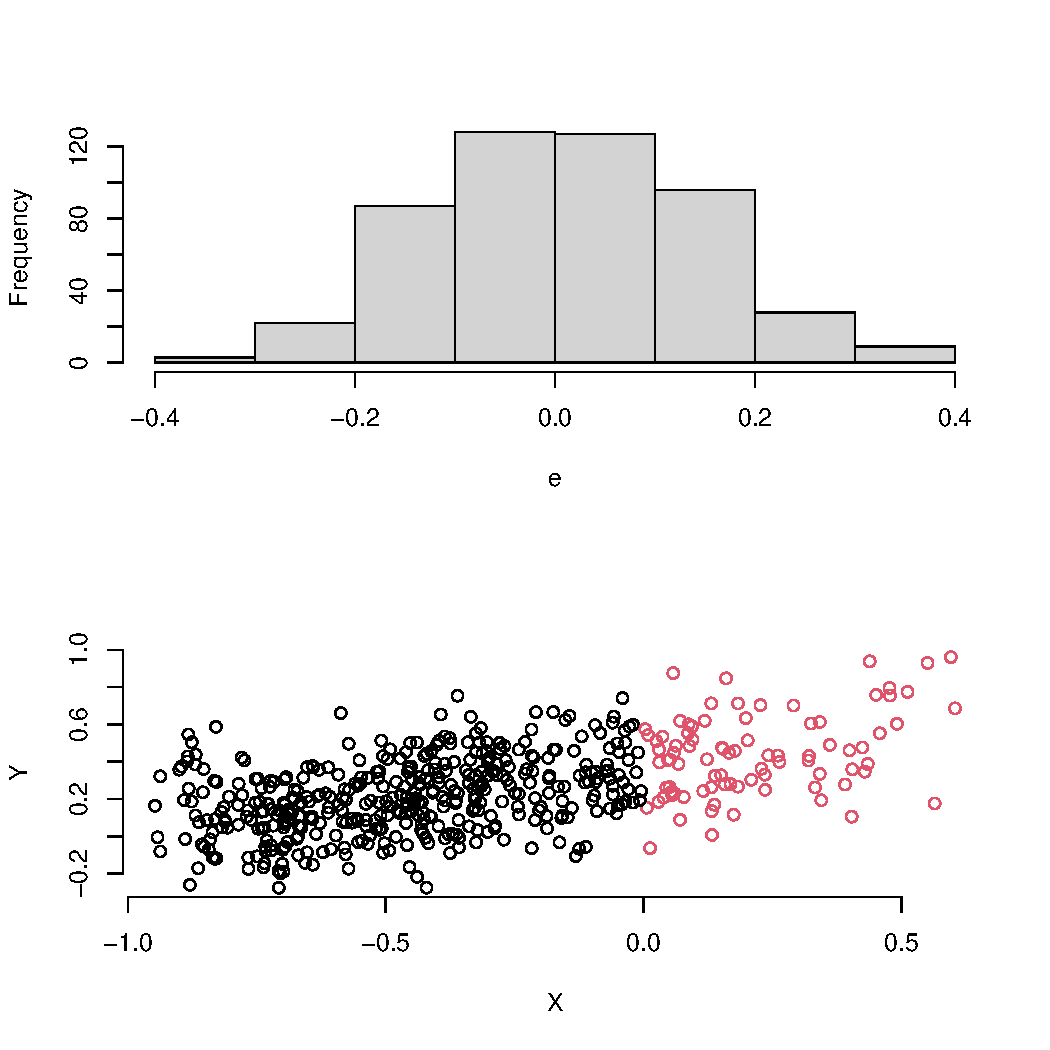
\includegraphics[width=.9\linewidth]{KR2023.pdf}
\end{center}

\subsubsection{Reguly2021}
\label{sec:org9afb512}
\cite{reguly2021heterogeneous} fits a CART model to additional
covariates and performs node-level polynomial regressions on
X. He takes 1000 samples of each DGP and considers \(n \in
\{1000,5000,10000\}\). Importantly, he samples \((X,W)\) only
once so that the variation across MCMC samples comes only
from \(\varepsilon\) and his treatment effect function
includes only \(W\) and not \(X\).

\begin{enumerate}
\item DGP 1:
\begin{itemize}
\item \(X \sim U(-1,1)\)
\item \(W_1,W_2 \sim \text{Bernoulli}(0.5)\)
\item \(\mu(x) = 2x\)
\item \(\tau(w_1) = 2 w_1 - 1\)
\item \(\varepsilon \sim \mathcal{N}(0,1)\)
\end{itemize}
\item DGP 2:
\begin{itemize}
\item \(X \sim U(-1,1)\)
\item \(W_1,W_2 \sim \text{Bernoulli}(0.5)\)
\item \(W_3,W_4 \sim U(-5,5)\)
\item \(\mu(x,w) = (4 w_2 - 2) x\)
\item \(\tau(w_3) = 2 w_3\)
\item \(\varepsilon \sim \mathcal{N}(0,1)\)
\end{itemize}
\item DGP 3 (variation of Lee data):
\begin{itemize}
\item \(X \sim 2 \mathcal{B}(2,4)-1\)
\item \(W_1 \sim \text{Bernoulli}(0.5)\)
\item \(\mu(x,w_1) = 0.48 + w_1(1.27 x + 7.18 x^2 + 20.21
     x^3 + 21.54 x^4 + 7.33 x^5) +(1-w_1)(2.35 x +
     8.18 x^2 + 22.21 x^3 + 24.14 x^4 + 8.33 x^5)\)
\item \(\tau(x,w_1) = w_1(0.02 - 0.43 x - 10.18 x^2 - 12.22
     x^3 - 12.53 x^4 - 3.77 x^5) + (1-w_1)(0.07 - 1.14 x -
     11.08 x^2 - 15.22 x^3 - 14.13 x^4 - 3.77 x^5)\)
\item \(\varepsilon \sim \mathcal{N}(0,0.05)\)
\end{itemize}
\item DGP 4 (variation of LM data)
\begin{itemize}
\item \(X \sim 2 \mathcal{B}(2,4)-1\)
\item \(W_1 \sim U(5,9)\)
\item \(\mu(x) = 3.71 + 2.30 x + 3.28 x^2 + 1.45 x^3 + 0.23
     x^4 + 0.03 x^5\)
\item \(\tau(w_1) = -0.45 + 16.19 x - 58.09 x^2 + 72.85 x^3 - 45.25
     x^4 + 9.8 x^5 - w_1\)
\item \(\varepsilon \sim \mathcal{N}(0,0.05)\)
\end{itemize}
\item DGP 5: DGP 3 of \cite{calonico2014robust}
\end{enumerate}

This is what the DGPs look like\footnote{DGP 3 and 4 look different from the paper. The former
looks similar when using smaller sample sizes and the
conversion from \(\mu_0,\mu_1\) to \(\mu,\tau\) is correct. The
latter had a typo in the paper so the one written here is a
guess. I could not find the simulation codes for the paper
to check this}:

\begin{center}
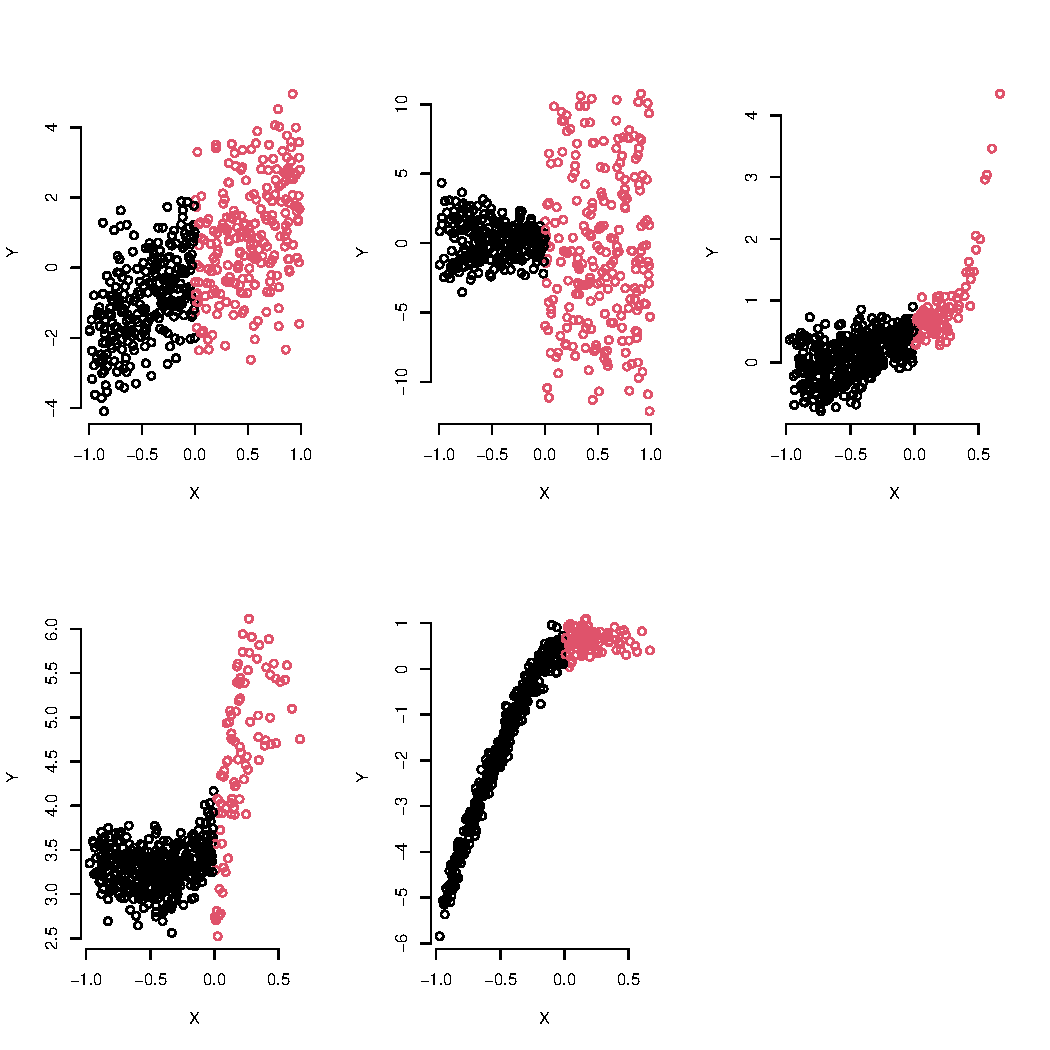
\includegraphics[width=.9\linewidth]{reguly.pdf}
\end{center}

Two things to note about this exercise. In DGP 1, we have
\(\tau(w=1) = 1\), \(\tau(w=0)=-1\) and \(E[\tau]=0\). It might be
interesting to include a case with zero ATE but some
non-zero CATE to be estimated in our setup. In DGP 2, a
similar thing happens but now with continuous CATE. The way
\(\tau\) is constructed is such that the continuous \(W\)
introduces huge variability in it, this is something to keep
in my mind when writing these simulations.

\clearpage
\bibliographystyle{apalike}
\bibliography{../../../Dropbox/References/references}
\end{document}